\begin{bibunit}
\thispagestyle{plain}

\section*{Abstract}
A rigorous check is a significant phase in the design process of control programs of safety-critical cyber-physical systems. Here, we consider such programs to be implemented using IEC~61499 standard for industrial automation. After the check is performed (for example, using formal verification), the engineer needs to ensure that even in unexpected situations, the system will not fail during the runtime, and for this online verification methods can be utilized.

In this work, we consider attaching monitors implemented as basic function blocks to the interface of the controller, thus having a property being monitored represented in the form of a state machine. Now, monitors make the system safer only if their quality is also ensured. Since their complexity is far lower than the complexity of the controller, they can be model checked, however, in the case of IEC~61499 function blocks, open-loop model checking will produce spurious counterexamples as it will allow combinations that are not possible according to the IEC~61499 function blocks semantics (e.g., data transferred without firing the event). The current work addresses this issue and proposes a method for close-loop model checking of monitors, using the non-deterministic twin of a controller under supervision. We present our approach using the system of two orthogonal pneumatic cylinders.

\section{\textsc{Introduction}}
%\PO{Continuing the topic of monitors in 61499 systems and their verification started in (Pranay, Monitoring design pattern for distributed automation systems in IEC 61499 and its formal modelling )}

%\PO{oflfine (static) verification of online (runtime) means for ensuring safety. }

%\PO{Works rarely cover testing of their observing mechanisms}

%\PO{There exist methods for monitoring IEC 61499 and methods for verifuinf IEC 61499, however there's none on verifying the monitors, which requires an interaction withthe system (?) }

%A rigorous check of safety-critical cyber-physical systems is crucial to industrial automation. 
Safety-critical cyber-physical systems must always comply with their requirements before they become operational. One of the important parts of the process of ensuring compliance is checking whether the control program (or controller) of such a system works as expected. This can be done using verification or validation approaches, which are united by the fact that none of them has a hundred percent coverage when dealing with complex industrial-sized systems. In the case of conventional testing or simulation, even if they are automated, some operational environment-related events might be left out and the industrial-sized system might be too complex to have all the possible test cases generated. Formal verification techniques allow the engineer to check the whole state space of the system; however, they suffer from a state-space explosion problem and of being computationally demanding overall when verifying complex systems. To combat this issue, various model abstraction techniques were developed to decrease model complexity (for example, to verify some particular functionality)~\cite{clarke2000,burch1992symbolic}. Another approach is bounded model checking, in which the executions of particular lengths are checked~\cite{biere2003bounded}. This, in turn, brings us back to the problem of missing a longer scenario that leads to failure.

Nevertheless, both approaches avail in finding the issues in the pre-operational stage, and what has to be added is an entity that would observe whether the particular property of the system holds during the runtime and communicate to an error handling system if the malfunction occurs. Such entities are called monitors or observers~\cite{17jhunjhunwala2022monitoring}. They can be internal or external to the system and perform the \emph{online verification}. Online verification has another advantage, i.e., if the changes have to be applied to the control program fast and there is a lack of resources to perform the global re-check, observers will maintain the safety state of the system by communicating the critical errors during the runtime.

In this work, our control programs are implemented following the IEC~61499 standard for industrial automation, and we consider internal monitors represented with basic function blocks, meaning that the properties of the system to be monitored are expressed as individual finite-state machines. This makes our monitors a better target for formal verification, and model checking, in particular, than the control program as a whole, since checking their whole state space requires less computational resources.

Model checking~\cite{clarke1999} is an approach for formal verification, where the formal model of the system is checked during the pre-operational stage, which is called \emph{offline verification}. In addition to a formal model of the system, model checking requires a formal representation of the properties of the system (for example, using linear temporal logic~(LTL)) as input. The model checker then derives all possible execution scenarios and produces counterexamples if the requirements do not hold. The counterexample for a requirement is such an execution scenario (or a system trace) where the requirement fails. 

Now, we propose to perform an offline verification (model checking) over the functional unit developed for online verification. Here, we face the issue that the traditional open-loop approach for model checking will produce spurious counterexamples due to the semantics of IEC~61499 function blocks~(FBs), where, for example, data cannot be sent or received without corresponding events being fired. 
We address this by modeling a non-deterministic twin of the controller and verifying a closed-loop model instead. We demonstrate our approach on a run-through example of two orthogonal pneumatic cylinders moving forward and backward. For model checking, we use NuSMV verifier~\cite{nusmv} and translate our FBs to its programming language (SMV) using the FB2SMV tool~\cite{drozdov2015fb2smv}.

The remainder of this paper is structured as follows. Section~\ref{sec:prelim} gives an overview of IEC~61499 standard and the verification methods of FBDs implemented according to it. Section~\ref{sec:method} describes a methodology for designing a supervised system, which is described in detail on a run-through example in Section~\ref{sec:methodappl}. Section~\ref{sec:concl} concludes the paper.

\section{\textsc{Preliminaries}}
\label{sec:prelim}
\subsection{IEC~61499}
IEC~61499 defines a design paradigm for distributed automation and control systems. The systems are implemented using the graphical language of function block diagrams~(FBDs). An FBD is a set of various interconnected FBs that can be of a basic, complex, or service interface type. In this work, we do not consider the latter. All FBs have their data and event input and output interfaces. The bricks of an FBD are basic FBs that represent atomic functional units. The logic of a basic FB is defined by an execution control chart~(ECC), which essentially is a Moore state machine and consists of states, transitions, and actions. In each state, an algorithm can be executed and/or an event (defined in the output interface of the FB) emitted. Complex FBs are nets of interconnected FBs of any type. The final FBD is assembled using the available FBs.

IEC~61499 systems are event-driven, unlike, for example, \mbox{IEC~61131-3}~\cite{tiegelkamp1995iec} systems that follow a cyclic execution pattern and \emph{event} is a key concept for the standard. Any event input or output can be bound to a subset of data inputs or outputs, respectively, which means that the corresponding data will be received and processed or sent only if the particular event fires. Intuitively, any update of the event variable opens the gates for the data connected to it.

In this paper, we create our observers using basic FBs, incorporating the logic of the condition to be monitored in their ECCs. As in~\cite{toolchain}, we use Non-Deterministic Transitions~(NDT) to create a non-deterministic twin of the controller of two pneumatic cylinders to verify the observers in a closed loop.



\subsection{IEC~61499 verification}
There exists a sufficient amount of literature on the topics of online (dynamic) and offline (static) verification of IEC~61499 FBDs. 

An overview of both static and dynamic verification approaches is given in~\cite{15blech2016comparison}.
\cite{12yoong2010verifying} proposes an approach of converting IEC~61499 FBs to Esterel and its subsequent verification.
In \cite{13yoong2015verification,14bhatti2011observer}, the monitors expressed as IEC~61499 FBs are added not for run-time verification but to better understand the counterexamples produced by the static verification approach. The system represented as a Kripke structure, together with observers and (possibly) computation tree logic~(CTL) formula are provided as input to the verification module. The authors suggest that, if the counterexample is received, the debugging process is simplified, as observers are inserted into the system structure.
\cite{11lindgren2016contract} considers static verification by enriching FBs with formal contracts and addressing verification on the component, algorithm, and ECC levels. In the works~\cite{agn_case_study} and~\cite{agnostic} the authors translate FBDs to SMV closed-loop formal models, \cite{toolchain} continues in this direction and presents a notation within IEC~61499 syntax for the subsequent generation of closed-loop formal models of FBDs and their verification by means of NuSMV. 


Examples of dynamic verification include, for example, \cite{1falcone2022runtime} that proposes adding enforcers to the application, which will not only monitor but adjust the supervised values in case of the property failure to ensure that the correct values are emitted by the controller. In~\cite{3do2020towards, 8ng2019contract}, the authors add assume and guarantee contracts in the form of FBs to the application to monitor the system during the run-time. \cite{4wenger15behavior} introduces behavioral runtime monitors into the 4DIAC framework. These monitors are generated automatically using service sequences extended with behavioral types. Combining various control and verification techniques, a reconfiguration architecture for fault handling in industrial systems is designed in~\cite{10leitao2020fault}. 


Approaches for dynamic and static verification, both, have their advantages and serve their purposes, hence, probably, the best way to ensure the system's correctness is to complement one with the other. However, despite the fact that there are numerous approaches for online verification, very few articles mention that the diagnosis units themselves must undergo a sanity check, which is especially important in relation to IEC~61499 FBs, where an occasional missing event in a transition condition can make a monitor erroneous. The point is outlined in~\cite{9wiesmayr2022supporting} and in~\cite{17jhunjhunwala2022monitoring} an approach to verify the monitors using Timed Net Condition-Event Systems was mentioned. We continue the work~\cite{17jhunjhunwala2022monitoring} and elaborate on the static verification of monitors expressed as IEC~61499 FBs and the challenges it brings. 
 
\begin{figure*}[htb]
    \centering
    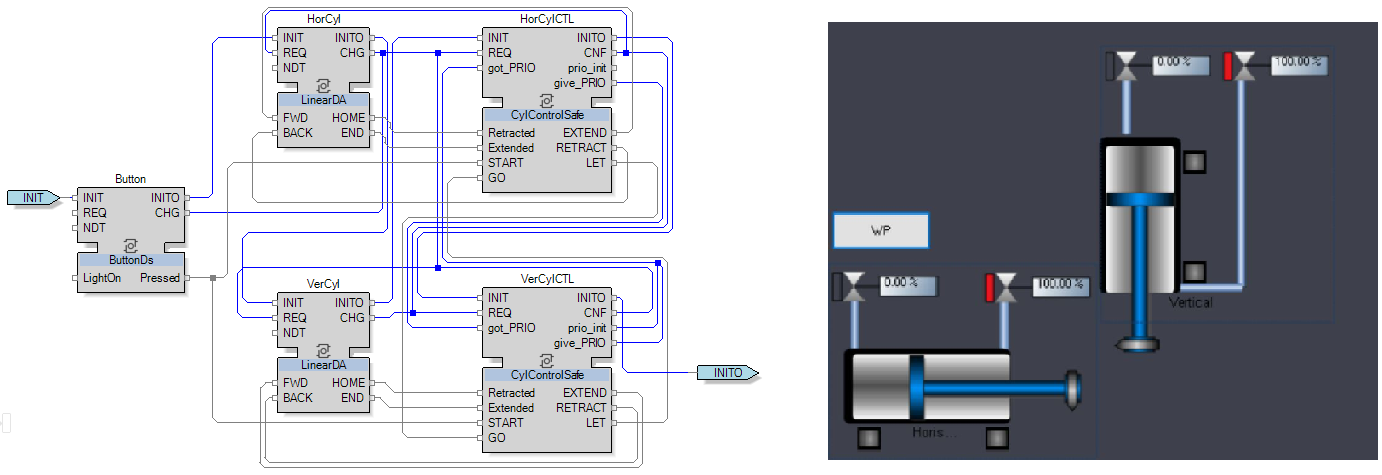
\includegraphics[width=0.98\textwidth]{MX_Papers/Paper3/pic/wholesystem_withhmi.png}
    \caption{The system of two pneumatic orthogonal cylinders. \texttt{HorCyl} and \texttt{VerCyl} simulate the plant (horizontal and vertical cylinder correspondingly), while \texttt{HorCylCTL} and \texttt{VerCylCTL} compose a control program. On the right, the HMI of the system is shown with the situation that should be avoided~-- a simultaneous extension of two cylinders.}
    \label{system}
\end{figure*}
%Tu t'es trompé de réseau de Pétri, le réseau où les deux cylindres ne se touchent pas c'est l'autre, tu l'as ou pas? 

\section{Design methodology for a monitored control program}
\label{sec:method}

For an automation system to function according to its specification, it must be checked using offline verification methods and equipped with online verification mechanisms to ensure that the requirements hold in unexpected circumstances. For this, the runtime verification means should also be checked.
Thus, in this paper, we propose a design methodology for the control programs implemented in form of IEC~61499 FBDs with internal observers (or monitors) that solves the aforementioned problem. Given a plant model (plant simulation program), for a single monitor, the methodology involves the following steps:
\begin{enumerate}
    \item Implementation of the control program.
    \item Verification of the control program in a closed loop with the plant model provided. Depending on its size, the plant model can be simplified and the heuristics for reducing the resulting closed-loop formal model state space may be applied. If the issues are found, the engineer has to address them and repeat this step until the verification result is positive.
    \item Formulation of a desired property to be observed in the form of a finite state machine and its implementation as a basic FB, i.e., implementation of the monitor.
    \item Implementation of the simplified non-deterministic twin of the controller that can produce any combination of outputs based on any combination of inputs. Verification of the created monitor in a closed loop with the twin. The properties to be formulated for the verification procedure, intuitively, are the following: the monitor indicates a failure when the failure occurs and the monitor does not report a failure when the controller functions as expected. If problems are found, they should be eliminated, and the system re-checked. This step should be repeated until the verification yields no counterexamples.
    \item Verification of the monitor in a closed loop together with the real control program.
    \item Verification of the monitor in a closed loop together with the control program where the fault was injected. Steps~5 and~6 may employ bounded model checking techniques or heuristics for state space reduction. The steps must be repeated if there were found issues to be addressed.
\end{enumerate}

The main contribution is concentrated in step~4.
In the next sections, we demonstrate our methodology step by step on a run-through example of a system of two pneumatic cylinders, especially focusing on step~4.


%As a base for our work, only one model is needed : an existing system. The first aim is to add a monitor to this model. The monitor added is not trustworthy, it has to be verified. 

%In order to avoid a kind of dependence to the current version of the system which needs to be checked, the monitor has to be verified independently. These formal verification have to ensure that the monitor would be able to output the correct result based on its inputs.\\
%In this paper, different kinds of formal verification of monitor will be approached. To prove and demonstrate that the method used is correct, we will use two systems with their behaviour verified. The first system is fully functional, while the second one is a dysfunctional analog of the first, with the error known. Those system are described in the Paragraph \ref{study_case}~~.

%For formal verification we used LTL expressions.

%The aim of this study is to reduce the number of checks of the entire system due to slight/little/minor modifications. Our idea is relies in the follows. Once the monitor is fully checked, it becomes trustworthy and able to check the behavior of the system instead of the formal verification.
%
%v2
%As a base for our work, only one model is needed: an existing system. The first aim is to add a monitor to this model. The monitor added is not trustworthy; it has to be verified. Different kinds of verification are needed to ensure that the monitor would work and would be able to verify our system. 
%The first verification considers the internal functioning of the monitor. A formal verification is applied to the monitor involving only its internal variables. The objective is to check the monitor's ability to output the correct result.
%The second verification is about its externals links. A second formal verification is applied to the monitor. This verification involves some of its internals variables and variable from the system. %pas clair
%The aim is to verify the functioning connections between the system and the monitor : its ability to correctly 'read' the working inputs.
%Once the monitor is fully checked, it is trustworthy and able to check the system's behaviour. This method allows us to avoid formal verification of entire systems and subsystems which would cost a significant amount of time especially for minor modifications.
%These formal verification are ensured thanks to LTL expressions.
%In this paper, to simplify the study at first, the system studied is a verified working system in order to ensure that mistakes only come from the monitor and not from the system. 
%To demonstrate the reliability of a formally verified monitor, this method will be applied a second time on the same system with behaviour modifications.
%The method described above will be applied a second time/once more with a dysfunctional system in order to prove the efficiency of the method. The dysfunctional system is the same model with voluntary dysfunctions that will be described in the following paragraph.
%
%v1
%As a base of our work, two models are needed : an existing model working as expected and the same existing model with voluntary dysfunctions. The first aim of adding same monitors to those models is to ensure that monitors work and are able to detect bugs that we have implemented. The systems are checked by Online verification.
%The second aim is to do formal verification of the models. LTL expressions have to contain variables from the working system and from the monitor. For the working model, the issue is to ensure that the monitor doesn't detect error which don't exist. For the dysfunctional model, LTL expression issue is to ensure that the monitor only detect errors. Once specification of LTL expressions are respected, it means that the formal verification from the system is the same as the formal verification of the monitor. The monitor is trustable.\\
%To confirm again the trustworthiness of monitors, systems studied here will be modified. The modifications applied do not have to change the main function of the system. Same process then will be applied to our modified system : multiple formal verifications with different LTL expressions. Finally, in the case of monitors and formal verifications outputting same 'things', it would proved the reliability of monitors checked with formal verification.
%This  verification is useful for more complex system. Offline verification is a real loss of time in the case of minor modifications. Limit of formal verification are not known thus this method implies to work with a simple model in order to avoid first endless calculations. 

\section {Methodology application}
\label{sec:methodappl}
\subsection{Steps 1 and 2: control program implementation and verification}

Our task was to create a control program for two orthogonal pneumatic cylinders that move towards each other and back by pressing a switch button. The plant simulation model was implemented as an IEC~61499 FBD in EcoStruxure Automation Expert (EAE).

The aim of the controller was to allow both cylinders to extend and retract once the button was pressed. The following safety requirement was to prevent the cylinders from colliding.
Thus, we implemented the priority system so that the horizontal cylinder can start moving only when the vertical cylinder is retracted. The complete system is presented in Figure~\ref{system}. Here, the control program consists of two controllers (for vertical and horizontal cylinders) of the same FB type that are connected in a closed loop with their plant models (cylinders). When the button is pressed, the command \texttt{START} is sent to the controllers and the cylinder with the higher priority gets the command to start its moving cycle (extend and retract). After the controller recognizes that its cylinder is retracted, it sends the priority giving event (\texttt{give\_PRIO}) to the vertical cylinder and sets the variable \texttt{LET} to true, allowing the vertical cylinder to take its turn.




%As it is stated in the Section~\ref{method}, there exist two versions of this system, i.e., correct and erroneous. Both of those systems are built using five Basic FBs. The first one is the controller(prev. switch?), once "pressed", it allows cylinders to move. Then, there are blocks that model the physical device of each cylinder (alternatively, we can call them plant blocks). They execute order of the command bloc such as "EXTEND", "RETRACT" or "STOP". Finally, there are command blocks of the horizontal cylinder and of the vertical cylinder. Those blocs receive information from the switch FB and send orders to the plant FB.
%The two cylinders are controlled and described the same way by the same FBs (same class but different objects).

%The most crucial requirement for our system is that the cylinders must never collide. Figure~\ref{system} shows the FB network of our correct system and its function is illustrated with a Petri net.\\
%Each cylinder has a priority, in our case, the priority of the vertical cylinder is higher than of the horizontal one. Therefore, when the button is pressed and both of variables \texttt{START} become \texttt{true}, the cylinder with a higher priority moves first. 
%In the end of its motion, the horizontal cylinder sends the priority giving event (\texttt{give\_PRIO}) to the vertical cylinder and sets the variable \texttt{LET} to true, allowing the vertical cylinder to take its turn.
%Thus, the system works in an infinite cycle. The system is forced in such a way that they cannot collide but neither are they able to extend a the same time no matter how many times the button is pressed.

In our case, the system is of a moderate size and we can apply model checking as is, without abstracting the system or using bounded model checking.
%To ensure that those models behave as expected, we model checked them using NuSMV verifier. 
Thus, we translated our system to SMV code using the FB2SMV tool and checked the following LTL formula with NuSMV verifier: \texttt{G $\neg$(Ver.EXTEND $\land$ Hor.EXTEND)} (where \texttt{Ver} and \texttt{Hor} are \texttt{VerCylCTL} and \texttt{HorCylCTL} correspondingly), 
%{\small$$G!(Ver.EXTEND=TRUE ~~\& ~~Hor.EXTEND=TRUE)$$}
which means that at every discrete time step, the two cylinders never get the command to extend simultaneously. The verification result was successful. 






%v1
%The method was implemented in the following case study: two perpendicular double-action cylinders commanded by a switch press button. The model is represented in Fig. 1. It is designed with IEC61499 standard through \textit{EcoStruxure Automation Expert (EAE)}.
%
%There are many different kinds of model of this system. First, we have the FB network which allows us to simulate with the HMI interface (Human Machine Interface) represented in Fig. \ref{petri_hmi_iec}(c). This model uses CAT FBs. CAT FBs are used to connect the Canvases objects in Fig. \ref{petri_hmi_iec}(b) and defined behaviours as forward and backward motion. They are plant FBs. However CAT FBs can not generate fbt files which are needed to do formal verification.
%Thus, we have a second FB network model allowing for a formal verification. CAT FBs are simply just substituted with basic FB also describing, thanks to ECCs, the forward and backward motion. These plant basic FBs' ECCs are built with NDT events which can be emitted at any time. It allows the formal verification to create many different combinations. \cite{toolchain} %of variables
%\\
%In both models, command of cylinders is controlled by basic FB. It is used to receive information from the switch press button and send information to the plant FB.
%The two cylinders are controlled and described by the same FBs (same class), with only objects being different.
%
%As said in the Method paragraph, we need two systems : the first one have to work perfectly and the other have to be dysfunctional. 
%The correct behaviour here is the case where cylinders never collide. Fig. \ref{petri_hmi_iec}(a) and \ref{petri_hmi_iec}(b) shows the FB network of our working system and it global operation illustrated with a Petri net.
%\\
%An order of priority has been defined upstream. During initialisation, the vertical cylinder gives priority to move to the horizontal cylinder. Once the switch button is pressed a 'START' signal is sent to the horizontal and to the vertical command FBs. To move, first, both cylinders need to have priority. Cylinder then will be in a waiting 'START' event state as it is shown in Fig. \ref{petri_hmi_iec}(b).

%Thus, the horizontal cylinder goes first. Just before the end of its motion, the command FB of the horizontal cylinder gives priority to the vertical cylinder letting it in the waiting 'START' event state and, at the end of its motion, sends a 'START' event: 'GO'\footnote{\label{GO}IEC 61499 rules does not allow two different outputs for a single data input. Another must therefore be created.} to the vertical cylinder, allowing it to move. 


%The system describes an infinite cycle where the horizontal cylinder moves first. Once the button is pressed it cannot be stopped. The system is forced in such a way that they cannot collide but neither are they able to extend a the same time no matter how many times the button is pressed.

%The dysfunctional system is different in terms of command FBs. There is no more priority rule. Once the switch button is pressed, the cylinders are both able to move at the same time and thus to collide as shown in Fig. \ref{petri_col}.
%both systems have
%The system has been checked firstly with HMI first and then with formal verification. Formal verification is described with the following LTL expression: 
%{\small$$G!(Ver.EXTEND=TRUE ~~\& ~~Hor.EXTEND=TRUE)$$}
%This means that for every combination of value of variables (G), the two cylinders never (!) extend at the same time. Expected behaviour has been observed, the LTL expression is always true in our assumed working system .
%and multiple counter-example have been found in our assumed dysfunctional system. 


\subsection{Step 3: Monitor implementation as a basic FB}


The next step was to create a monitor that would observe whether the safety property (i.e., two cylinders should never receive the command to extend simultaneously) is maintained by the system during the runtime. We implemented the monitor as a basic FB and assumed that it would be connected to the controllers as in Figure~\ref{fig:monitorplacement} (other connections are not depicted for the sake of clarity).

%The monitor has to observe the system the same way (as) the previous formal verification (did). This means that it has to check that the two cylinders never extend at the same time. 

\begin{figure}[h!]
    \centering
    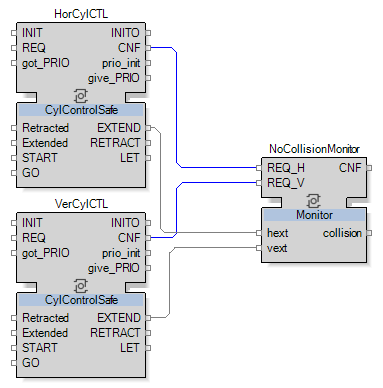
\includegraphics[width=0.35\textwidth]{MX_Papers/Paper3/pic/monitorplacement.png}
    \caption{Monitor \texttt{NoCollisionMonitor} connected to the controllers (other connections are not shown for clarity).}
    \label{fig:monitorplacement}
\end{figure}

%This monitor was implemented as a basic function block. 
The monitor receives the \texttt{EXTEND} outputs from both controllers together with their events \texttt{CNF} and communicates whether the collision is occurring by setting its output \texttt{collision} to \texttt{true} and triggering the \texttt{CNF} event. The ECC of the monitor is presented in Figure~\ref{fig:monitorecc}.

%Its ECC, Figure~\ref{ECC} is able to know (when and) which cylinder is extending. 'OBSERVER' FB only returns 'collision := TRUE' when the 'HextANDVext' state is reached.

%After multiple online tests with the functional systems, the monitor seems able to output a consistent result with our system behaviour.
%The monitor shown here can present mistakes, so it is susceptible to change depending on results of its formal verification.

\begin{figure}[h!]
    \centering
    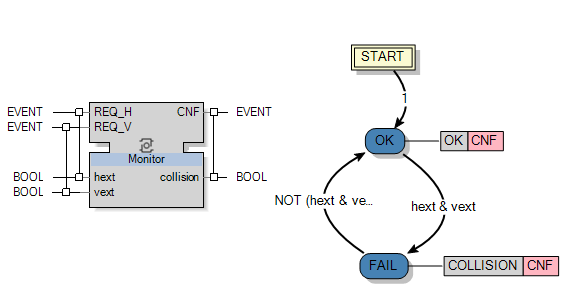
\includegraphics[width=0.48\textwidth]{MX_Papers/Paper3/pic/monitorecc.png}
    \caption{Interface of the monitor and its ECC. Algorithms \texttt{OK} and \texttt{COLLISION} set output variable \texttt{collision} to \texttt{false} and \texttt{true} correspondingly.}
    \label{fig:monitorecc}
\end{figure}

\subsection{Step 4: monitor verification with a non-deterministic twin of the controller }
\label{sec:monitorver}
The next step is to verify the implemented monitor in a closed loop with the controller (which we decompose into two controllers~-- for vertical and horizontal cylinders). In our case, the controllers are represented with basic FBs, and the closed-loop model checking will produce the result within an acceptable time interval. However, we will have to close the loop on the inputs of the controllers as well, meaning that we will either have to model simplified plants or provide other means for the controllers to produce all the possible combinations of their output values. Moreover, even if we succeed in closing the loop on the controllers, in case issues are found during the model checking, counterexamples will be hard to decipher as they will elongate and dozens of additional variables will be added to the system state.

Thus, we propose creating a \emph{non-deterministic twin} of the controller, which will be represented with two FBs of the same type just like our individual cylinder controllers. Now, let us disclose the notion of a non-deterministic twin~(ND twin). 

To model check the monitor, it is important that the model checker would infer all the possible combinations of its inputs, meanwhile triggering the events associated with them. Therefore, the goal of an ND twin is to abstract the logic of the controller by saving its key states, where the variables that are monitored change and add the non-deterministic transitions~(NDT) between them. Such events in an FBD turn into non-deterministic inputs in the SMV module of the corresponding FB, generated by FB2SMV as described in~\cite{agn_case_study}. 

The ECC of our individual controller of the cylinder together with its ND twin are presented in Figure~\ref{fig:ndtwinecc}. Two states that change the supervised variable \texttt{EXTEND} are \texttt{EXT}, \texttt{RETRACT}, and \texttt{STOP}. We kept them in the ND~twin and added NDTs between them so that at any time any output could be produced. From the algorithms, we remove everything that does not influence the variable \texttt{EXTEND} and leave only the \texttt{CNF} event associated with it. Figure~\ref{fig:ndtwinloop} shows two ND~twins of the controllers connected to our monitor.

\begin{figure}[t]
    \centering
    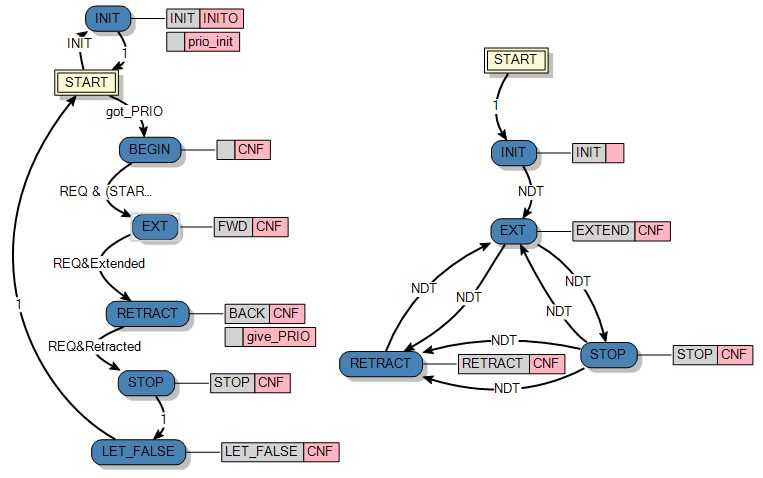
\includegraphics[width=0.5\textwidth]{MX_Papers/Paper3/pic/ndtcontrollereccs.png}
    \caption{ECCs of the cylinder controller (to the left) on of its ND~twin (to the right).}
    \label{fig:ndtwinecc}
\end{figure}


\begin{figure}[b]
    \centering
    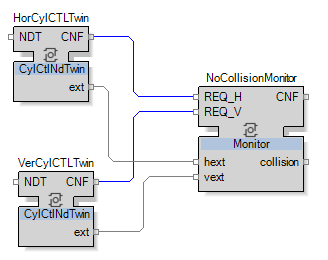
\includegraphics[width=0.34\textwidth]{MX_Papers/Paper3/pic/ndtwinloop.png}
    \caption{Connection of the monitor to ND~twins of the cylinder controllers.}
    \label{fig:ndtwinloop}
\end{figure}

When the system is converted to SMV, the first step is to verify that we can indeed get all the values of the monitor input, that is, our ND twins function according to their specifications. The set of properties that make up the specification can be created according to the following template. 

Assume that we have a set of all the supervised variables in a single ND~twin $U$.
$\forall u \in U, \exists D_u$, where $D_u$ is a domain of $u$. Then, $\forall u \in U, \exists V_u = \{(u,v) \:|\: v \in D_u\}$, where $V_u$ a set of all possible assignments of $u$. Now, a set of all the possible combinations of the variables values is $C = V_{u_1}\times\ldots\times V_{u_n}, n = |U|$. Having $C$, we can now formulate the CTL specifications to be checked as a set $S$:
$$S = \{\textbf{AG} \:\neg(\bigwedge_{p \in P} u(p) = v(p)) \:|\: P \in C\},$$
where $P$ a set of variable and value pairs, $u(p)$ returns the variable name of pair $p$ and $v(p)$ its value. Thus, if any of the specifications from $S$ are satisfied, it means that their corresponding combination cannot be generated by a formal model of an ND~twin.
Similarly, we check if the observer can get all the possible combinations of input values.

In our case, we checked the following specifications for the ND~twins (here, \emph{twin} is replaced with the corresponding names of the FBs for horizontal and vertical cylinders controllers twins): \texttt{AG twin.EXTEND} and \texttt{AG $\neg$twin.EXTEND},~-- and four specifications for the monitor of type \texttt{AG $\neg$(NoCollisionMonitor.hext $\land$ NoCollisionMonitor.vext)} (we omit others to save space). All the specifications failed, which means that all the combinations were possible in our model. 

Now, that we know that our model produces all the combinations of inputs, we can formulate the properties of the monitor to be checked. The first one tells that whenever the monitor gets the signals that both of the cylinders extend simultaneously, it produces the warning. Its LTL equivalent is: \texttt{\textbf{G} ((m.hext $\land$ m.vext) $\rightarrow$ (m.hext $\land$ m.vext \textbf{U} m.collision))}, where \texttt{m.} is short for \texttt{NoCollisionMonitor.}. Here we use operator \textbf{U}~-- ''until'' instead of \textbf{X} (''next'') or no temporal operator due to the specifics of the generated SMV model, where several model evaluations should occur to obtain the result of the FB output.

The second property tells that if the cylinders are not extending simultaneously, the collision is not reported, which is in LTL: \texttt{\textbf{G} ($\neg$(m.hext $\land$ m.vext) $\rightarrow$ \textbf{F} $\neg$ m.collision)}.

Both properties were satisfied by our monitor.

%A new solution has been provided in this paper. Formal verification of the monitor alone could not deal with connections and it is hard to understand how formal verification emits the different event and datas of the monitor. To meet the needs of it, a new system is created and modeled. This system would be a kind of a twin of the original system able to create every possible case. A first version is designed.\\

%\begin{figure}[h!]
%    \centering
%    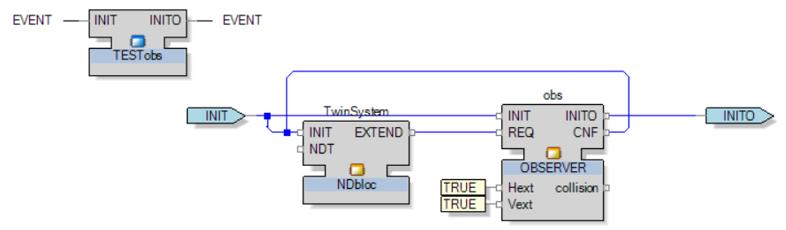
\includegraphics[width=0.48\textwidth]{MX_Papers/Paper3/pic/jumeau_V1.png}
%    \caption{First version of the twin two cylinders system}
%    \label{twin1}
%\end{figure}

%The twin system is composed of two FBs. The first one is the monitor and the other one is a simple basic FB able to output, thanks to a 'NDT' event, a 'EXTEND' event directly connected to the event 'REQ' of the monitor. moreover, datas of the monitor are forced as TRUE as seen in Figure~\ref{twin1}. Those 2 blocks are implemented in a composite FB and composed its FB network.\\
%During the formal verification, the event 'NDT' will be emitted randomly which will activate the 'REQ' event and thus the datas. LTL expression used here is the~(\ref{LTLmonitor}) one. A counterexample is found.

%As seen in the counterexample visualizer (Figure~\ref{vizu_twin1}), the monitor is still stuck in the 'OnlyH' state whereas Hext and Vext datas become TRUE at the same time. The twin system has to be improve but it already allows us to find some mistakes in the monitor. In facts, if the two datas become TRUE at the same time, in the ECC, it does not exist any transition for this case. Transitions are added. Then, if the system is stuck it's also because it can' read correctly transitions. The 'REQ' event is emitted once for two datas. It needs to be split into two different input events each will be link to one of the two datas. 'REQ\_h' is created and connected to 'Hext' and 'REQ\_v' is created and connected to 'Vext', Fig. \ref{monitorV2}.\\
%Now that two 'REQ' events have been created, a another bloc is added to the system in order to also trigger one of the 'REQ\_h/v ' event. A second version of the twin system is designed (Figure~\ref{twin2}).

%\begin{figure}[h!]
%    \centering
%    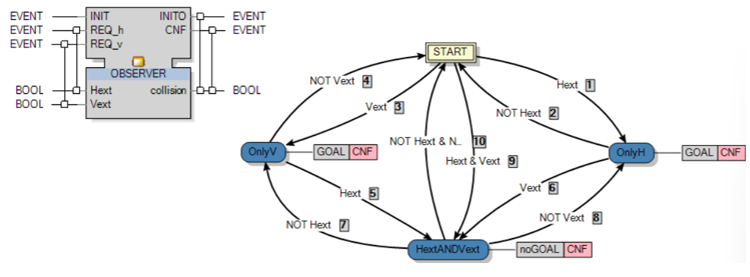
\includegraphics[width=0.48\textwidth]{MX_Papers/Paper3/pic/mointorV2.png}
%    \caption{Monitor and its ECC modified}
%    \label{monitorV2}
%\end{figure}

%A new formal verification is done, same LTL expression. Another counterexample, Figure~\ref{vizu_twin2}, is found. However, if watched more closely, the monitor is able to output that a collision happen but after few steps. Those few steps represent only steps needed to reach the good state and the time to activate the action allowing the monitor to output 'collision=TRUE'. The monitor here seems to work but to be more specific and make the formal verification founds no counterexample, the LTL expression needs to be modify. Using the function 'F', for future, would allows to reach our goal. The LTL expression now becomes :
%\begin{center}
%    $G(~(OBS.Hext = TRUE~~\&~~OBS.Vext = TRUE)$\\
%\end{center}
%\begin{equation}
%    \xrightarrow~~\textit{\textbf{F}}~~OBS.collision = TRUE)
%    \label{LTLmonitor2}
%\end{equation}


\subsection{Steps 5 and 6: monitor verification with the real and erroneous controller}

Now, we add the monitor to the system and check whether we connected it properly by verifying the system with the monitor as a whole. If the system at step~2 was checked using state-space reduction techniques, they can be applied here as well.

To check whether the monitor works when there is an error in the system, we inject the fault manually. In our case, we remove the priority mechanism from the controllers so that, by pressing the button, both cylinders extend simultaneously. The ECC of the erroneous cylinder controller is shown in Figure~\ref{fig:errctlecc}.

With both systems, we partially verify the same properties as in Section~\ref{sec:monitorver}. In both cases, we check whether all combinations of input values are possible for the monitor. The correct system reports that there is no possibility for two cylinders to get the extension command simultaneously, while only this is possible in the malfunctioned system. Then, we check the monitor properties, i.e., whether it reports the collision when it happens and does not report spurious collisions. Since the collision is not allowed in the first system, we omit the first monitor property, when checking the correct system, similarly, we omit the second property, checking the erroneous one. In both systems the checked properties hold, thus we can conclude that the monitor and its connections are correct.


\begin{figure}[t]
    \centering
    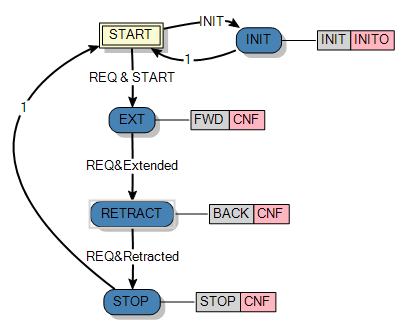
\includegraphics[width=0.34\textwidth]{MX_Papers/Paper3/pic/errctlecc.png}
    \caption{The ECC of the erroneous cylinder controller.}
    \label{fig:errctlecc}
\end{figure}

%Now it's to see if the monitor is still working while implemented in the correct model and the erroneous one. A new formal verification is made. No counterexample has been found in both model. The monitor is verified formally.




%The dysfunctional version of the described system is different in terms of command FBs. There is no more priority rule. Once the switch button is pressed, the cylinders are both able to move at the same time and thus to collide as shown in Figure~\ref{HMI_collide}.

%\begin{figure}[h!]
%    \centering
%    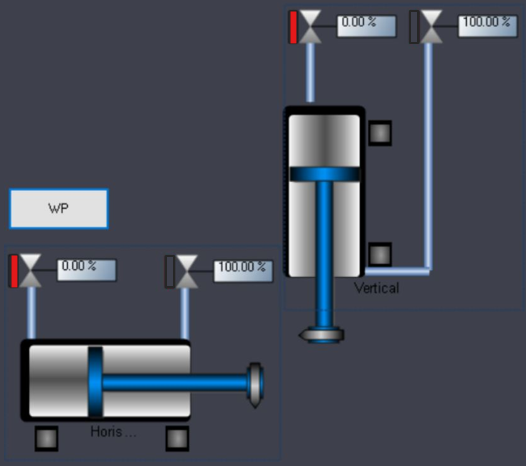
\includegraphics[scale=0.5]{MX_Papers/Paper3/pic/HMI_collide.png}
%    \caption{HMI representation of the two cylinders system colliding}
%    \label{HMI_collide}
%\end{figure}

%Monitor works online but there could be a transition path where a failure could appear. These paths can be determined with formal verification. The main aim of the monitor formal verification is to ensure that its internals are correctly designed. Misconceptions inside the monitor FB could be detected, i.e., an unreachable state.

%As said in the Section~\ref{method}, the monitor has to be checked independently from the system it has to observe. The first way to do it is to do the formal verification of the monitor alone. Indeed, from its own .fbt file, it is possible to do a formal verification. This formal verification would only involve internal inputs and outputs events and/or datas of the monitor ECC.\\
%The LTL expression has to verify the ability of the monitor to output the correct result depending on inputs. The LTL expression and its opposed should verify all the different cases.
%\begin{center}
%    \textit{G( (OBS.Hext = TRUE~~\&~~OBS.Vext = TRUE)}
%\end{center}
%\begin{equation}
%    \xrightarrow~~OBS.collision = TRUE)
%    \label{LTLmonitor}
%\end{equation}\\
%It means every time (G), if inputs \textit{Hext} and \textit{Vext} are true then the output \textit{collision} must be true.

%As a result, the LTL expression is always true, no counterexample has been found. This result allows to make a conclusion : the monitor works as expected.

%To see if it's true and if this kind of formal verification of monitors is enough to demonstrate that monitors are trustworthy, the monitor was added to both versions of the system (correct one and erroneous ones).\\
%When implemented in the functional system, checked with the same LTL expression~(\ref{LTLmonitor}), no counterexample is found. However, the system is functional so collision never happens. CHECK THIS It means that only the opposed of the LTL expression \ref{LTLmonitor} has been checked here, which is LTL expression~(\ref{LTLopposed}).
%\begin{center}
%    $G(OBS.collision = FALSE)$
%\end{center}
%\begin{equation}
%    ~~\xrightarrow~~(OBS.Hext = FALSE~~OR~~OBS.Vext = FALSE)
%    \label{LTLopposed}
%\end{equation}

%When implemented in the erroneous system, formal verification founds mistakes. Indeed, when the two cylinders are extending, the monitor is not able to output that there is a collision. Thanks to the counterexample of the visualizer, Figure~\ref{vizu_dys}, it is possible to understand what happen. Actually, the monitor is stuck in the 'OnlyH' state which outputs "no collision". Lots of hypothesis about the source of the problem but from now only a conclusion about this formal verification can be done: the formal verification of monitor only based on their .fbt file is not enough.



%The monitor works online but there could be a transition path where a failure could appear. These paths can be determined with formal verification.
%\\
%The main aim of the monitor verification is to ensure that its internals are correctly designed. Misconceptions inside the monitor FB could be detected by formal verification ie an unreachable state.
%
%In our case, the monitor FB is a basic FB so it is defined and composed by ECC.
%
%\subsubsection{Internal behaviour}
%First, only doing the formal verification of the monitor has been thought.\\
%This formal verification would only involve internal inputs and outputs events and/or datas of the monitor ECC and would be done directly from the \textit{fbt} file  of the monitor.
%\\
%The LTL expression has to verify the ability of the monitor to output the correct result. 
%LTL expression (ECC monitor alone)
%\begin{center}
%    {\footnotesize $G ((OBS.H\_ext = TRUE~~\&~~OBS.V\_ext = TRUE)$}\\
%    {\footnotesize$\xrightarrow~~OBS.collision = TRUE)$}
%\end{center}
%It means every time (G), inputs \textit{H\_ext} and \textit{V\_ext} are true then the output \textit{collision} must be true.
%\\
%As a result, the LTL expression is always true. It means that the ECC of the monitor works as expected.
%\\

%\subsection{Connections verification}
%However, the aim of a monitor is not to work alone, it has to be implemented. Moreover, the previous verification can not permit to conclude about the real behaviour of the monitor. In facts, to be fully checked, the monitor has to be simulated in a system which able to submit all the different possibilities of input combinations.
%
%A new system is created Fig. \ref{twin}. The aim is to recreate a simplified copy of the original system allowed to generate non deterministic events. Thanks to those non deterministic events and the NuSMV tool, the system will be able to generate all the different possibilities of input combinations.
%It composed of three basic FBs. One of them is the monitor. The two other FBs are twin of the cylinders command FBs. They are based on the same FB.
%\\
%As a basic FB, it is described by an ECC shown in Fig. \ref{ECC_twin}. Non deterministic events allows the state machine to evolve between its several states. The transition are called non deterministic transitions (NDT).
%\\
%When the \textit{'NDstate'}, for non deterministic state, is reached, the FB outputs the variable \textit{'EXTEND'} as true. Those outputs are directly connected to the observer bloc, one to \textit{'H\_ext'} and one to \textit{'V\_ext'}. The \textit{'EXTEND'} variable value is reset after that a second ND event (NDT2) is emitted.
%\\
%A quick online verification is made to ensure that the result is the same as the first online check in \textit{IV.B}.
%
%The system is verified offline with the following LTL expression :
%\begin{center}
%    {\footnotesize $G ((HorTwinCTL.EXTEND = TRUE~~\&~~VERTwinCTL.EXTEND = TRUE)$}
%    {\footnotesize$\xrightarrow~~F~~obsTEST.collision = TRUE)$}
%\end{center}
%
%This LTL means that every time (G) the \textit{'EXTENT'} variable of both basic FBs is true then the variable %\textit{'collision'} of the observer must be true instantly or in some states later (F).
%
%As a result, NuSMV finds counter-examples of this LTL expression. Which means that our monitor displays misconceptions.
%After being tested with all the different possibilities of inputs in a similar system, We thought our monitor could be considered as a certified working one.



%%%%%%%%%%%%%

%The monitor is 
%A first LTL expression has been test : 
%\begin{center}
%     {\footnotesize $G ((HorCTL.EXTEND=TRUE~~\&~~VerCTL.EXTEND=TRUE)
%     \xrightarrow ~~  (obs.collision=TRUE))$}
%\end{center} 
%But it return counters example. In fact, this LTL expression pretends that the detection of the monitor is instantaneous. In the detail of counter-example file, it is because the monitor detects the error several state after the two cylinders extend(ed/ing) at the same time. Therefore, we tried another approach :
%\begin{center}
%    {\footnotesize $G ((HorCTL.EXTEND=TRUE~~\&~~VerCTL.EXTEND=TRUE)
%     \xrightarrow~~$}
%     {\small $F(obs.collision=TRUE))$}
%\end{center}

%It means that the detection will arrive in the future (F) or, in other words, several states after the both EXTEND signals (verical and horizontal) came true . The potential drawback is that the detection arrive too late, but this can't be quantify in this case. Nevertheless, it is a starting point to avoid the previous issue. After implement this formula in Nusmv, it return that the LTL statement is TRUE.  

%%%%%%%%%%%%%%%%



%\subsection{Monitor implemented in the working system}
%\vspace{0.2cm}
%Now, the aim is to ensure that the monitor is correctly implemented in the system. The formal verification permits to test the connections of the monitor with the system. 
%\\
%The verification condition of our system is simple so are the connections between the system and the monitor. As said in the section \textit{B. Adding monitor} from the paragraph \textit{IV. STUDY CASE}, the monitor only reclaims two outputs from the command FB of each cylinder. A simple connections is needed (fig. \ref{monitor}). With the same LTL expression schema, this condition is checked.
%
%LTL expression (system+monitor in S)
%\begin{center}
%     {\footnotesize $G ((HorCTL.EXTEND=TRUE~~\&~~VerCTL.EXTEND=TRUE)
%     \xrightarrow ~~  F (obs.collision=TRUE))$}
%\end{center} 
%
%
%explanation of the expression
%This expression means : "IF the horizontal cylinder is extending AND (\&) if the vertical cylinder is also extending THEN ($\rightarrow$) the monitor must always (G) return "collision=TRUE". 
%\\
%It return that this LTL expression is always true.
%
%However, the system known as a working system, the variable 'EXTEND' of both cylinder can not be TRUE at the same time. Thus the LTL expression is not directly verified, only is its contraposition :
%\begin{center}
%    {\footnotesize $G(obs.collision=FALSE) \rightarrow~~$}\\ 
%    {\footnotesize $!~(HorCTL.EXTEND=TRUE~~\&~~VerCTL.EXTEND=TRUE)$}
%\end{center}
%
%\begin{figure}[h!]
%    \centering
%    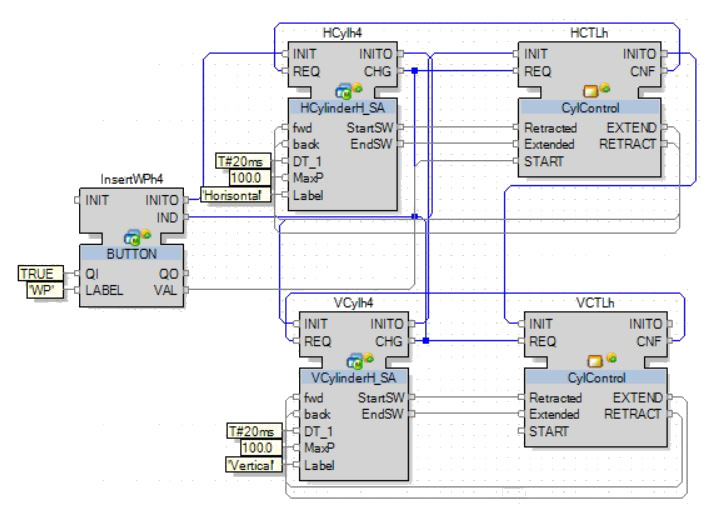
\includegraphics[width=0.45\textwidth]{MX_Papers/Paper3/pic/IEC_syst_col.JPG}
%    \caption{IEC model design of the two cylinders able to collide}
%    \label{IEC_collide}
%\end{figure}

%\subsection{Monitoring with modifying the system} 
%\vspace{0.2cm}
%ajouter une transition pour dire que ca marche avec un system modifié en tout cas inchallah
%
%Now that monitor ECC is working and connections with the system are correctly established, our monitor is trustworthiness and able to fully diagnose online systems errors. To prove it, let's implement our monitor in a slightly different system.   
%\\
%The previous part assure that the monitor does not detect false error. However, we don't know is behaviour when it's linked to a system which include misconceptions.   
%
%Thus, we introduced a different system.
%it's actually the same as previously but with behaviour modifications.
%
%idée d'Etienne : il vient pas de poitier, permettre au système d'ateindre tout les états possible (ie même ceux "interdits") 
%
%Il n'a pas detecté d'erreur inexistante mais on ne l'a pas confronté à un système pouvant comporter des erreurs. Certe, ses entrèes sont cohérentes avec ses sorties (cf première LTL) mais (sinon on a juste à s'arréter à la vérif du ECC tout seul)) pas ouf 
%
%Nous avons vérifié les connections avec un système qui marche, nous avons vu que ces connections ne créent pas de fausses erreurs mais permettent-elles d'en detecter? c'est ce que nous allons voir en l'ajoutant à un système comportant des erreurs.
%
%
%
%%It is different in terms of command FBs. There is no more priority rule. Once the switch button is pressed, the cylinders are both able to move or not at the same time and thus to collide. As seen in Fig. \ref{IEC_collide}, the model design is almost the same and Fig. \ref{petri_collide} represented its Petri net.
%\\
%\begin{figure}[h!]
%    \centering
%    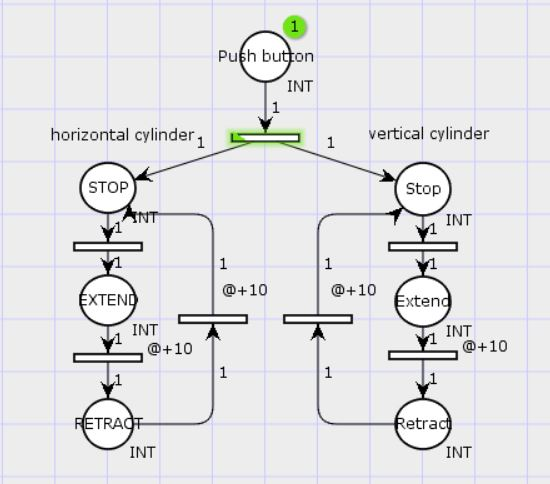
\includegraphics[width=0.3\textwidth]{MX_Papers/Paper3/pic/systeme_col.JPG}
%    \caption{Petri net  model of the two cylinders able to collide}
%    \label{petri_collide}
%\end{figure}
%
%% implementation of the monitor and online verification of the system
%The monitor is implemented in this system. It is connected the same way as it was in the previous %system : the monitor reclaims the 'EXTEND' variable from the horizontal and the vertical %cylinders (Fig. \ref{monitor} and Fig. \ref{IEC_collide}).
%%The monitor and its connections with the system, identically as before,  does not need any %formal verification. Pas compris
%
%Online verification may be run with the modified system. The monitor finds out that, at some %point, the two cylinders are extending at the same time. 
%\\
%If it sticks to the method plan, mistakes should come from the system - the monitor tells the %truth. To confirm this hypothesis, the system and the system with the monitor have to be %checked thanks to formal verification.
%
%FV of the system but no HMI verification just offline
%The system has been first checked alone - including only variables from the system. Formal %verification is described with the same LTL expression as the first system :
%{\small$$G!(Ver.EXTEND=TRUE ~~\& ~~Hor.EXTEND=TRUE)$$}
%
%Expected behaviour has been observed, the LTL expression is false, a counter-example file have %been returned with the expected mistake.
%\\
%
%Online, with adding the monitor, it can detect the simultaneous extend.
%\\
%However, when the monitor was added to the formal verification with the following LTL %expression : (the same as the working system)
%
%\begin{center}
%     {\footnotesize $G ((HorCTL.EXTEND=TRUE~~\&~~VerCTL.EXTEND=TRUE)
%     \xrightarrow ~~  F (obs.collision=TRUE))$}
%\end{center} 
%
%Then, NuSMV return a counter-example, not as expected. Therefore, our simplified system with all the possibility as to be reconsidered.

\section{Conclusion and future work}
\label{sec:concl}

In this paper, we presented a design methodology for the supervised system implemented in form of IEC~61499 FBD, putting special attention to the verification of the supervision mechanisms, that is, the monitors. This methodology allows using formal verification with state-space reduction or abstraction techniques while verifying the system as a whole, while creating reliable means for online observation of its function. Our main contribution is the approach for extensive closed-loop verification of monitors implemented in form of IEC~61499 FBs using the simplified non-deterministic twins of the controllers.

Having the system monitored gives an additional advantage while introducing small changes to the system when, for instance, the time does not permit performing the whole recheck. If the connections to the monitor do not change, with the proper setting of an error handling unit, the system will stay safe even if the new change leads to a failure.

The manual implementation of the proposed methodology may seem to cost time and effort; however, the process can be automated. Our future work in this direction focuses on creating the plugin to an open-source IDE for IEC~61499 programs, FBME~\cite{fbme}, that would implement the algorithm that distinguishes the key states of the controller, which change the variables under supervision, and generate a FB with NDTs between such states (i.e, ND~twin). The properties that should be checked on an SMV model of an ND~twin can also be generated automatically following the definition that we used in the current work. Thus, if we assume such a plugin, the input data for it would be a monitor, a supervised controller, and a set of temporal properties with which the monitor should comply. The subsequent check of the monitor injected into the system as a whole can be done semi-automatically, depending on the size of the SMV model of the system. 


Another direction of future work is to explore the scalability of our monitor-checking approach and verify more complex properties that include not only inputs of the monitors but any variable in the system, as well as monitors and controllers implemented as composite FBs.

%In our case, formal verification of the twin system is from 5.000 to 10.000 times faster than the formal verification of the entire system
\section*{Acknowledgments}
%\PO{This work was supported?} 

This work was supported, in part, by the HORIZON 2020 project 1-SWARM funded by the European Commission (grant agreement: 871743) and Horizon Europe project Zero-SWARM funded by the European Commission (grant agreement: 101057083).

We also wish to thank Dr. Igor Buzhinsky for suggesting us the missing piece of the puzzle during the work on Section~\ref{sec:monitorver}.

\putbib
\end{bibunit}
